% IEEE standard conference template; to be used with:
%   spconf.sty  - LaTeX style file, and
%   IEEEbib.bst - IEEE bibliography style file.
% --------------------------------------------------------------------------

\documentclass[letterpaper]{article}

% custom setup

% Folder for images
\graphicspath{{images/}}

% set pdf attributes
\usepackage[pdftex,
pdftitle={A Descriptive Title, no too general, not too long},
pdfauthor={Fabian Wuethrich, Jonas Hansen, Pascal Huber},
pdfkeywords={ETH, Fastcode, ASL, Fractal Image Compression}
]{hyperref}


% Title.
% ------
\title{A Descriptive Title, not too general, not too long}
%
% Single address.
% ---------------
\name{Jonas Hansen, Pascal Huber, Fabian Wüthrich\thanks{Janis Peyer for his contributions}}
\address{Department of Computer Science\\ ETH Zurich, Switzerland}

% For example:
% ------------
%\address{School\\
%		 Department\\
%		 Address}
%
% Two addresses (uncomment and modify for two-address case).
% ----------------------------------------------------------
%\twoauthors
%  {A. Author-one, B. Author-two\sthanks{Thanks to XYZ agency for funding.}}
%		 {School A-B\\
%		 Department A-B\\
%		 Address A-B}
%  {C. Author-three, D. Author-four\sthanks{The fourth author performed the work
%		 while at ...}}
%		 {School C-D\\
%		 Department C-D\\
%		 Address C-D}
%

\begin{document}
%\ninept
%
\maketitle
%

\begin{abstract}
    Fractal image compression provides is a lossy image compression scheme,
    which yields good compression ratios and quality at the cost of high encoding times.\\
    In our work, we started with our own implementation of a fractal compression scheme using quadtree partitioning
    and exhaustive search for self-similarity in the image. 
    We then applied various optimizations to the given computations, such as ILP, precomputation and vectorization using AVX2 intrinsics.\\
    Our optimized version without SIMD led to a 3x speedup, whereas we observed a speedup of up to 8x with vectorization.
    \notejonas{speedups anpassen}
    \notejonas{mehr details was wir gemacht haben}
\end{abstract}

\section{Introduction}\label{sec:intro}
Human perception relies heavily upon visual information, particularly images.
This medium is very powerful in gaining and conveying \textit{ideas}, memories,
and emotions. No one would doubt the saying
\begin{quote}
A picture is worth a thousand words.
\end{quote}
With the advent of social media and new image classification algorithms based on
neural networks, the ability to share and store images efficiently is crucial.
This imposes a wide range of challenges from storing sweet cat pictures to
transfer massive training data sets for medical image analysis.

\notepascal{too many ML details?}

A practical way to store images without occupying too much space is to use lossy
image compression which decreases the image quality in places where a
high-quality image is not perceivable or where an image of lower quality is not
disruptive. JPEG, whose basic building block is the discrete cosine transform,
is undoubtedly the most widely used lossy compression scheme. With good
compression quality and fast compression times, JPEG hits a sweet spot for many
practical applications.

Fractal image compression is another method for lossy image compression. The
main idea is to compress an image by exposing self-similarity which can be
observed in many places in nature (e.g. fir cones or romanesco broccoli).

Contrary to JPEG, the underlying theoretical construct of a fractal compression
scheme is that of an iterated function system (IFS). This approach yields great
compression results in terms of compression size and quality \cite{fisher2012}.
However, it is computationally expensive to encode images because the algorithm
involves an exhaustive search over different regions of the image (section
\ref{sec:background}) with many numerical computations to find self-similarity.
Optimizing these computations is therefore crucial for an efficient
implementation of the algorithm.

\mypar{Related work} The most widely known practical fractal compression scheme
was developed and patented by Michael Barnsley and Alan Sloan in 1987. They
published a paper about their work in 1989 \cite{barnsley1989fractal}. Barnsleys
graduate student Arnaud Jacquin was the first who implemented a practical
version of it in 1992 in his PhD thesis \cite{jacquin1990fractal}. Numerous
improvements and variations have then been developed to this original approach,
e.g. archetype classification (\cite{jacobs1992image}, \cite{boss1991studies})
which decreases the exhaustive search space for self-similarity. Yuval Fisher
published a book in 2012 with a detailed description of various fractal schemes
and an elaborate list of optimizations \cite{fisher2012}.

\mypar{Contribution} Based on the explanations of Fisher in \cite{fisher2012}
and an open-source implementation in Python \cite{github-python} and C++
\cite{github-cpp}, we implemented our own fractal image compression scheme with
quadtree partitioning and exhaustive self-similarity search.

In our work, we did not focus on algorithmic optimizations, but optimized the
computations of a given algorithm as best as we could.

\section{Background}\label{sec:background}

To introduce the algorithm, we first present the essential parts of the
underlying mathematical theory, show how it can be used to compress images and
what practical considerations must be made for the implementation. A cost
analysis can be found at the end of this section. Throughout this chapter, we
use the notation and results from Fisher \cite{fisher2012}.

\mypar{Iterated Function Systems (IFS)} Fractal image compression builds on the
theory of iterated function systems. For completeness, we provide a short
introduction to this rich topic.

\begin{definition}[Contractivity of Functions]
    A function $f$ on a metric space $X$ with metric $d$ is contractive, when there exists some $0 \leq k < 1$
    such that for all $x,y \in X: d(f(x), f(y)) \leq k \cdot d(x,y)$.
\end{definition}

As an informal example, when $f$ is a contractive function on $\R$, then mapping
two numbers brings them \textit{closer} together, i.e. their distance gets
smaller.

\begin{definition}[Iterated Function System]
  An iterated function system (IFS) is a set of $n$ functions
  \begin{align*}
    \{f_i:X \to X | i=1,\ldots,n\}
  \end{align*}
  where each $f_i$ is contractive and $X$ is a metric space.
\end{definition}

\begin{definition}[Hutchinson Operator]
    The Hutchinson operator for an IFS is the function
    \begin{align*}
        F \colon 2^X &\to 2^X\\
        x &\mapsto \bigcup_{i=1}^n f_i(x)
    \end{align*}
\end{definition}

With $F^{\circ n}(x)$, we denote the iterative application of $F$ $n$ times on
its input $x$, e.g. $F^{\circ 2}(x) = F(F(x))$.

\begin{definition}[Attractor of an IFS]
    Let $A \in X$. When $F(A)=A$, then $A$ is called an attractor.
\end{definition}

Hutchinson used the following theorem in his work \cite{hutchinson1981fractals}
to build up the essential theoretical parts of how fractal image compression works.

\begin{theorem}[Contractive Mapping Fixed-Point Theorem]\label{theorem-fixpoint}
  For an IFS on a compact set $X$ it holds that:

  \begin{enumerate}[topsep=0pt,itemsep=-1ex,partopsep=1ex,parsep=1ex]
    \item There always exists a unique attractor $A \in X$
    \item For any nonempty set $S_0 \subset X$ it holds that
      $A = \lim_{n \to \infty} F^{\circ n}(S_0)$
  \end{enumerate}
\end{theorem}

\mypar{From IFS to Image Compression} The key idea in fractal image compression
is that one computes a set of contractive functions $w_i \in \boldsymbol{W}$ (in
this context called transformations) on the image. From theorem
\ref{theorem-fixpoint}, we know that some unique attractor $A$ exists. If the
transformations $\boldsymbol{W}$ are chosen in a way such that the attractor $A$
is the image to be compressed, one only needs to store the transformations. For
decompression, one can iteratively apply all transformations on any initial
starting image, which then converges towards the original image.

A transformation $w_i$ is defined on a contiguous source region (called domain
block) and a contiguous target region (range block) of the image. The
transformation maps the pixels of the domain block to the pixels of the range
block and then applies a brightness and saturation adjustment.

The transformations can then be computed with the following steps.

\begin{enumerate}[topsep=0pt,itemsep=-1ex,partopsep=1ex,parsep=1ex]
  \item Partition the image into range blocks $\boldsymbol{R}$ and domain blocks
    $\boldsymbol{D}$.
  \item For each range block $R_i \in \boldsymbol{R}$, find a transformation
    $w_i$ with domain block $D_i \in \boldsymbol{D}$ such that $w_i(D_i)$
    approximates the pixel values of block $R_i$ best.
\end{enumerate}

Finding the best transformation by comparing all domain/range block pairs is
called exhaustive block mapping. More elaborate versions like archetype
classification restrict possible domain block candidates for a given range block
to speed up compression \cite{jacobs1992image}.

\mypar{Transformations} A grayscale image can be interpreted as a function
\begin{align*}
    f \colon I^2 &\to I\\
    (x,y) &\mapsto z = f(x,y)
\end{align*}

where $I$ is the interval $[0,1]$. Specifically, an image is a set of three-tuples $(x,y,z) \in I^3$, where $x,y$ are positions and $z$ is the grayscale value.
The image of a range (or domain) block $R_i$ is then defined by $f \cap (R_i \times I)$.
A transformation $w_i$ from the image of a domain block $D_i$ to the image of a range block $R_i$ can then be described as a linear affine transformation
\begin{align*}
w_i(D_i) = \bigcup_{(x,y,z) \in f \cap (D_i \times I)} \begin{pmatrix} a_i & b_i & 0 \\ c_i & d_i & 0 \\ 0 & 0 & s_i \end{pmatrix} \begin{pmatrix} x\\y\\z \end{pmatrix} + \begin{pmatrix} e_i\\f_i\\o_i \end{pmatrix}
\end{align*}

where $a_i, b_i, c_i, d_i, e_i, f_i$ map \textit{location} (which can involve rotations) and $s_i, o_i$ correspond to contrast and brightness adjustments.
To ensure that $w_i$ is contractive, $D_i$ has to be larger than $R_i$ (in terms of region sizes) and $0 \leq s_i < 1$.

Now we define a metric to compare two images (or two blocks). Usually, the root mean square error (RMS) metric is used:
\begin{align*}
d_{RMS}(f,g) = \sqrt{\int_{I^2} (f(x,y)-g(x,y))dxdy}
\end{align*}
For a range block $R_i$ and domain block $D_i$ we now seek the best
transformation $w_i$:
\begin{align}
  w_i = \argmin_{w} \left( d_{RMS}(w(D_i), f \cap (R_i \times I)) \right)\label{eq:min-problem}
\end{align}

Calculating $w_i$ is a minimization problem, because we may choose $s_i$ and
$o_i$ in order to minimize the error.

The set of all transformations is a partitioned iterated function system (PIFS).
The only difference to an IFS is that the transformations are restricted to
\textit{blocks} (partitions) of the image. However, the underlying theory still
holds \cite{fisher2012}.

\mypar{Computing Transformations}\label{par-practical-implementation}
In practice, an image consists of pixels, where each pixel has a grayscale value between 0 and 1 and integer coordinates.

The minimization problem in equation~\eqref{eq:min-problem} can be solved using least squares regression, as done in \cite{github-python}.
Fisher uses an analytical solution in \cite{fisher2012} to compute the adjustments directly. Let $b_1, ..., b_n$ be the $n$ pixel values of the range block $R_i$
and $a_1,...,a_n$ be the $n$ pixel values of the downsampled and rotated domain block. We then seek $s$ (saturation) and $o$ (brightness) such that
\begin{align*}
  R = \sum_{i=1}^n (s \cdot a_i + o - b_i)^2
\end{align*}
is minimal. An analytical solution for $s,o,R$ is:
\begin{align}
    s &= \frac{n \sum_{i=1}^n a_i b_i - \sum_{i=1}^n a_i \sum_{i=1}^n b_i}{n \sum_{i=1}^n a_i^2 - \left(\sum_{i=1}^n a_i \right)^2} \label{contrast}\\
    o &= \frac{1}{n} \left( \sum_{i=1}^n b_i - s \sum_{i=1}^n a_i \right) \label{brightness}\\
    R &= \frac{1}{n} \left[ \sum_{i=1}^n b_i^2 + s \left( s \sum_{i=1}^n a_i^2 - 2 \sum_{i=1}^n a_i b_i + 2o \sum_{i=1}^n a_i \right) \right. \notag\\
    &\text{\hspace{1cm}} \left. + o \left(no - 2 \sum_{i=1}^n b_i \right)  \right]\label{error}
\end{align}
Computing these values is the core numerical challenge of the algorithm.

\mypar{Image Partitioning} There are many ways to partition an image into range
and domain blocks. We require that the range blocks cover the full image and do
not overlap, otherwise the decompressed image would have uncovered regions. The
domain blocks represent the search space for self-similarity and may overlap.
Increasing the domain block pool $\boldsymbol{D}$ may lead to superior
transformations but can increase the compression time significantly. Blocks can
be of various sizes and shapes (quadratic, rectangular, etc.), but domain blocks
must be larger than range blocks to satisfy the contractivity requirement. For
example, the code in \cite{github-python}, uses quadratic range blocks of size
$s \times s$ and domain blocks of size $k\cdot s \times k \cdot s$ for some
integer constant $k > 1$.

\mypar{Quadtree Partitioning} In practice, quadtree partitioning is considered
a reasonable reference point for more advanced partitioning schemes
\cite{fisher2012}. It dynamically adapts range and domain block sizes by a
predefined error threshold $\epsilon$. We start with some initial (quadratic)
range blocks of size $s \times s$, and domain blocks of size $2s \times 2s$.
When there is a range block for which all domain blocks exceed the threshold
$\epsilon$, we partition the range block into 4 smaller blocks of size
$s/2 \times s/2$ and try to cover them again with domain blocks of size
$s \times s$. This scheme has the effect that (potentially larger) homogeneous
regions of the image are covered with few transformations while image regions
with details are covered with transformations that map smaller blocks. Usually,
one defines also a maximum depth of the quadtree as described in
\cite{fisher2012}.

\mypar{Cost Analysis} In this course, we focus on floating point operations and
ignore all integer calculations (e.g. index computation). We count only floating
point multiplications, divisions, additions, and subtractions because no special
mathematical functions are used. The cost metric is defined as
\begin{align}
  C = N_{mult} + N_{div} + N_{add} + N_{sub} \label{eq:cost}
\end{align}

The cost of the algorithm does not only depend on the size but also on the content
of an image. To obtain a rough estimate of the runtime, we provide a
pessimistic upper bound on the cost of the algorithm. We assume that no transformation
will yield an error below the threshold and thus the only termination criteria is the
maximum quadtree depth. In practice, the cost is (much) lower assuming a reasonable
error threshold $\epsilon$.

Let $m$ be the maximum quadtree depth and let $s$ be the width of the square
input image. We assume that we start quadtree with range blocks of size
$\frac{s}{2}\times\frac{s}{2}$ and one domain block of size $s \times s$. For
quadtree depth $i \in \{1, \dots, m\}$, let $R^{(i)}$ be the set of range
blocks, $D^{(i)}$ the set of domain blocks and $n_{i}$ the number of pixels of
one range block. Note that the number of pixels of a domain block is then always
$4\cdot n_{i}$ due to quadtree partitioning and $n_i=\frac{s^2}{|R^{(i)}|} = \frac{s^2}{2^{2i}}$.
For a given domain block and range block in quadtree depth $i$,
let $\alpha_{i}$ denote the cost to compute four transformations $w_i^{0}$,
$w_i^{90}$, $w_i^{180}$, $w_i^{270}$ and their errors. Each transformation
$w_i^{\gamma}$ represents a rotation of the domain block by $\gamma$ degrees.

To calculate $\alpha_{i}$, we need to compute all sums for brightness
\eqref{brightness}, contrast \eqref{contrast} and error \eqref{error} and apply
the formulas. Besides, we need to downscale and rotate the domain block.

Downscaling one domain block can be done in $4\cdot n_{i}$ flops because we have
to aggregate the average of four pixels of the domain block into one pixel which
requires 4 flops for every square of four pixels.

The sum $\sum_{j=1}^{n_{i}} a_j b_j$ has to be computed for each rotation which
requires $2\cdot n_{i}-1$ flops per rotations. The results of the remaining sums
($\sum_{j=1}^{n_{i}} a_j$, $\sum_{j=1}^{n_{i}} a_j^2$,
$\sum_{j=1}^{n_{i}} b_j$,$\sum_{j=1}^{n_{i}} b_j^2$) are identical for all four
rotations and and require a total of $6\cdot n_{i}-4$ floating point operations.
Applying the formulas for brightness, contrast and the error involves $26$ flops
using the precomputed sums. Therefore,
\begin{align*}
  \alpha_i &= 4\cdot n_{i} + 4 \cdot (2\cdot n_{i}-1) + (6\cdot n_{i}-4) +  26\\
           &= 18\cdot n_{i} + 18 \\
           &= 18 \cdot \frac{s^2}{2^{2i}} + 18
\end{align*}
Thus, we get the following upper bound on the cost:
\begin{align*}
C &\leq \sum_{i=1}^m |R^{(i)}| \cdot |D^{(i)}| \cdot \alpha_i \\
  &= \sum_{i=1}^m 2^{2i} \cdot 2^{2i-2} \cdot (18 \cdot \frac{s^2}{2^{2i}} + 18) \\
  &= \frac{6}{5}\cdot (4^{m}-1)\cdot (4^{m+1} + 5\cdot s^{2} + 4)
\end{align*}
We see that the cost of the algorithm is exponential in the quadtree depth $m$
and polynomial in image width $s$. For the roofline plot and the other benchmarks,
we determined the cost empirically by instrumenting the code.

\section{Your Proposed Method}\label{sec:yourmethod}

Now comes the ``beef'' of the paper, where you explain what you
did. Again, organize it in paragraphs with titles. As in every section
you start with a very brief overview of the section.

For this course, explain all the optimizations you performed. This mean, you first very briefly
explain the baseline implementation, then go through locality and other optimizations, and finally SSE (every project will be slightly different of course). Show or mention relevant analysis or assumptions. A few examples: 1) Profiling may lead you to optimize one part first; 2) bandwidth plus data transfer analysis may show that it is memory bound; 3) it may be too hard to implement the algorithm in full generality: make assumptions and state them (e.g., we assume $n$ is divisible by 4; or, we consider only one type of input image); 4) explain how certain data accesses have poor locality. Generally, any type of analysis adds value to your work.

As important as the final results is to show that you took a structured, organized approach to the optimization and that you explain why you did what you did.

Mention and cite any external resources including library or other code.

Good visuals or even brief code snippets to illustrate what you did are good. Pasting large amounts of code to fill the space is not good.
\section{Results}\label{sec:exp}

In the first part of this section, we describe the benchmark infrastructure and the
images we used for the measurements. Then we analyze how different compilers and flags
affect the performance of our code. In the end, we discuss each optimization and compare
them in different plots.

\mypar{Experimental setup} All benchmarks and tests were conducted on an Intel
Core i7-8650U processor with \textit{Intel Turbo Boost} disabled, running at 1.9
GHz. The CPU has a 4$\times$32 KB 8-way associative L1 cache, a 4$\times$256 KB
4-way associative L2 cache and 4$\times$2 MB 16-way associative L3 cache
\cite{intel-opt-manual}.

We used the peak signal-to-noise ratio (PSNR) to ensure that our baseline implementation
compresses the image correctly. This metric is widely applied to compare an image with its
compressed version. Typical values for the PSNR range from 25 to
50 dB (higher is better). The same metric was used to verify that the optimizations
produced the same result as the baseline.

The PSNR of the compressed image depends on the maximum depth $m$ of the quadtree and the error
threshold $\epsilon$. We set $m=7$ and $\epsilon=300$ for all our experiments. These parameters
produced an image of good quality in a reasonable amount of time.

We chose to benchmark our algorithm with a challenging image depicting a lioness
with its cub \cite{lions}.
While some parts of the image, for example the
background, are easy to compress, other parts such as the fur contain lots of details,
which are harder to compress. Figure \ref{fig:lions} shows the output of the
vectorized code with $\epsilon=100$ and 3 decompression iterations.

\begin{figure}[]
  \centering
  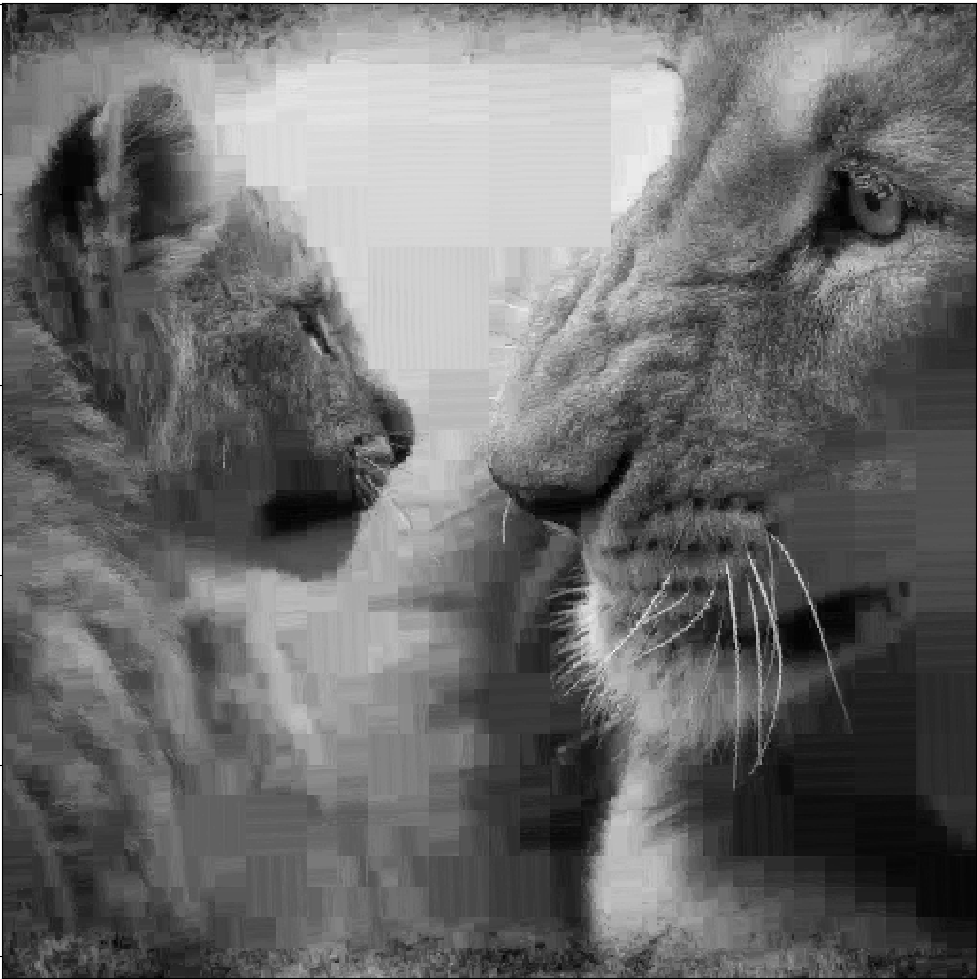
\includegraphics[page=1, width=.8\linewidth]{lion_512_51_e100}
  \caption{Decompressed Image}\label{fig:lions}
\end{figure}

\mypar{Compiler Flags} Several benchmarks were conducted comparing the achieved
performance using different compiler flags for the \textit{GNU Compiler
  Collection (gcc)} version 9.3.0 and the \textit{Intel C++ Compiler (icc)}
version 19.1.1.217. For all tests \texttt{-march=native} was set.

For both the scalar and the vectorized versions the flag \texttt{-O1} increased
performance significantly. While \texttt{-O2} did improve the scalar
implementation (figure \ref{fig:perf_scal}), it did not make a difference for
the vectorized version (figure \ref{fig:perf_vec}). Neither \texttt{-O3} nor
\texttt{-Ofast} were able increase performance for both code versions.

\begin{figure}[H]
  \centering
  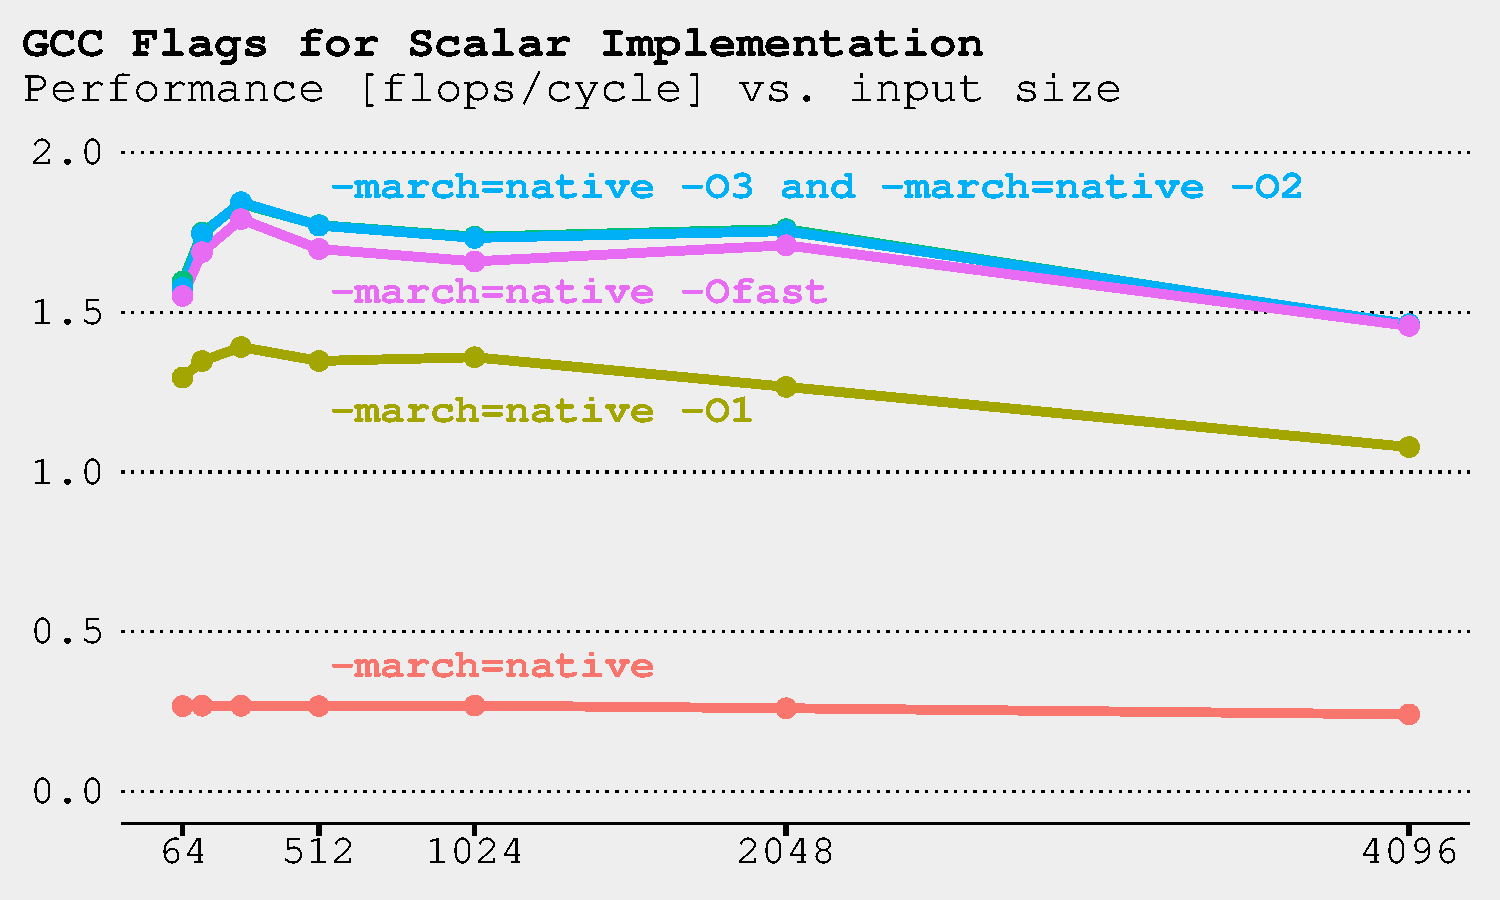
\includegraphics[page=1, width=\linewidth]{performance_scalar_opts}
  \caption{Performance of the four major GCC optimization flags for the scalar
    implementation}\label{fig:perf_scal}
\end{figure}

\begin{figure}[H]
  \centering
  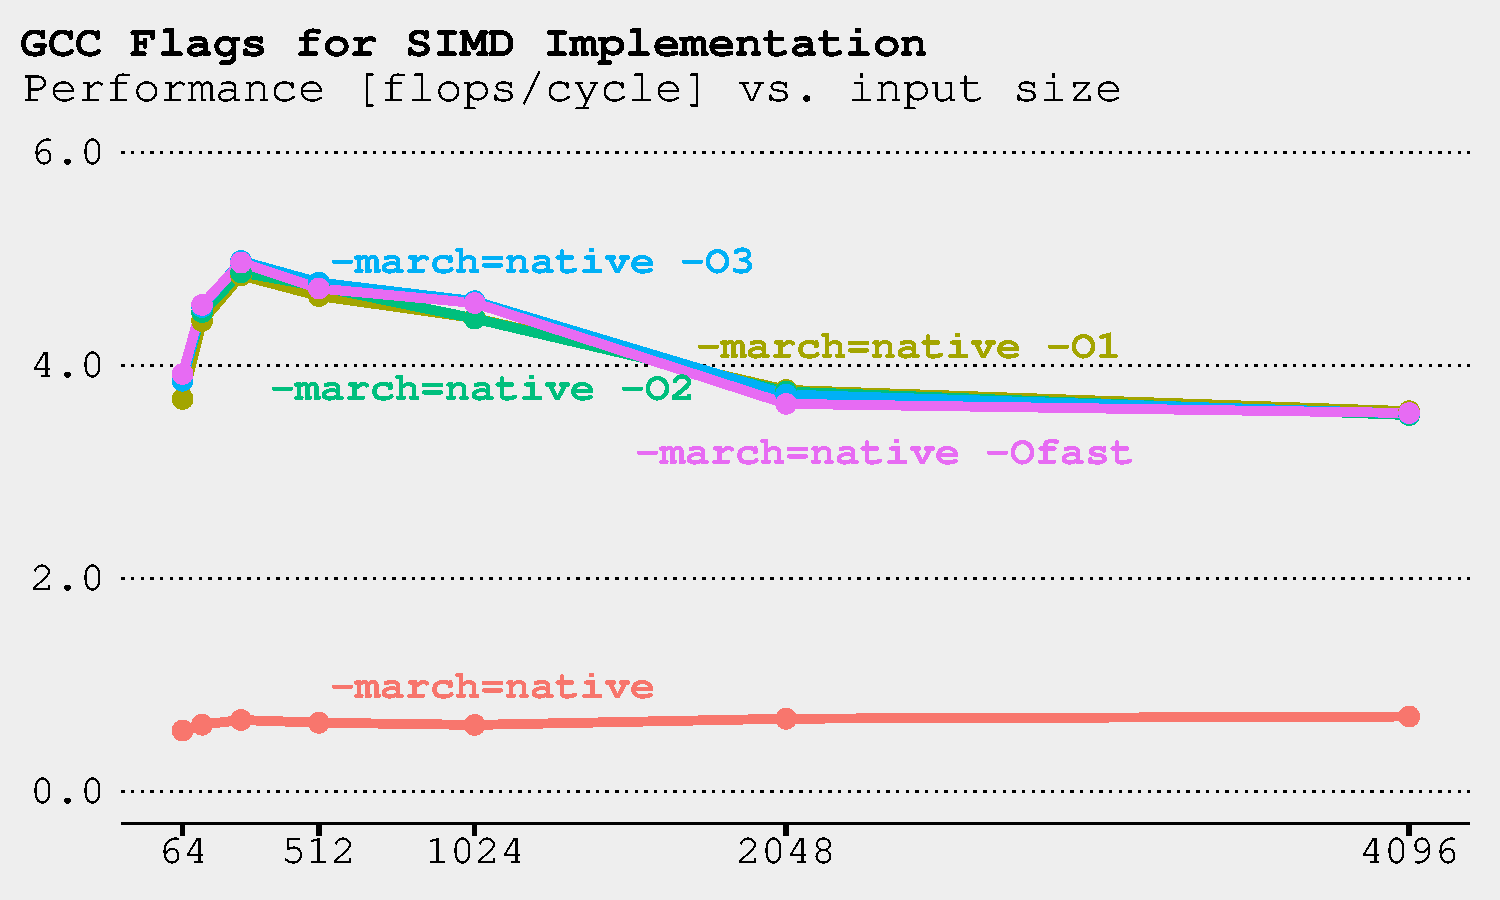
\includegraphics[page=1, width=\linewidth]{performance_vectorized_opts}
  \caption{Performance of the four major GCC optimization flags for the vectorized implementation}\label{fig:perf_vec}
\end{figure}

Intel's compiler was not able to outperform gcc but at least for the vectorized
version it managed to keep up for the larger images as shown in figure
\ref{fig:perf_gcc_vs_icc}.

\begin{figure}[H]
  \centering
  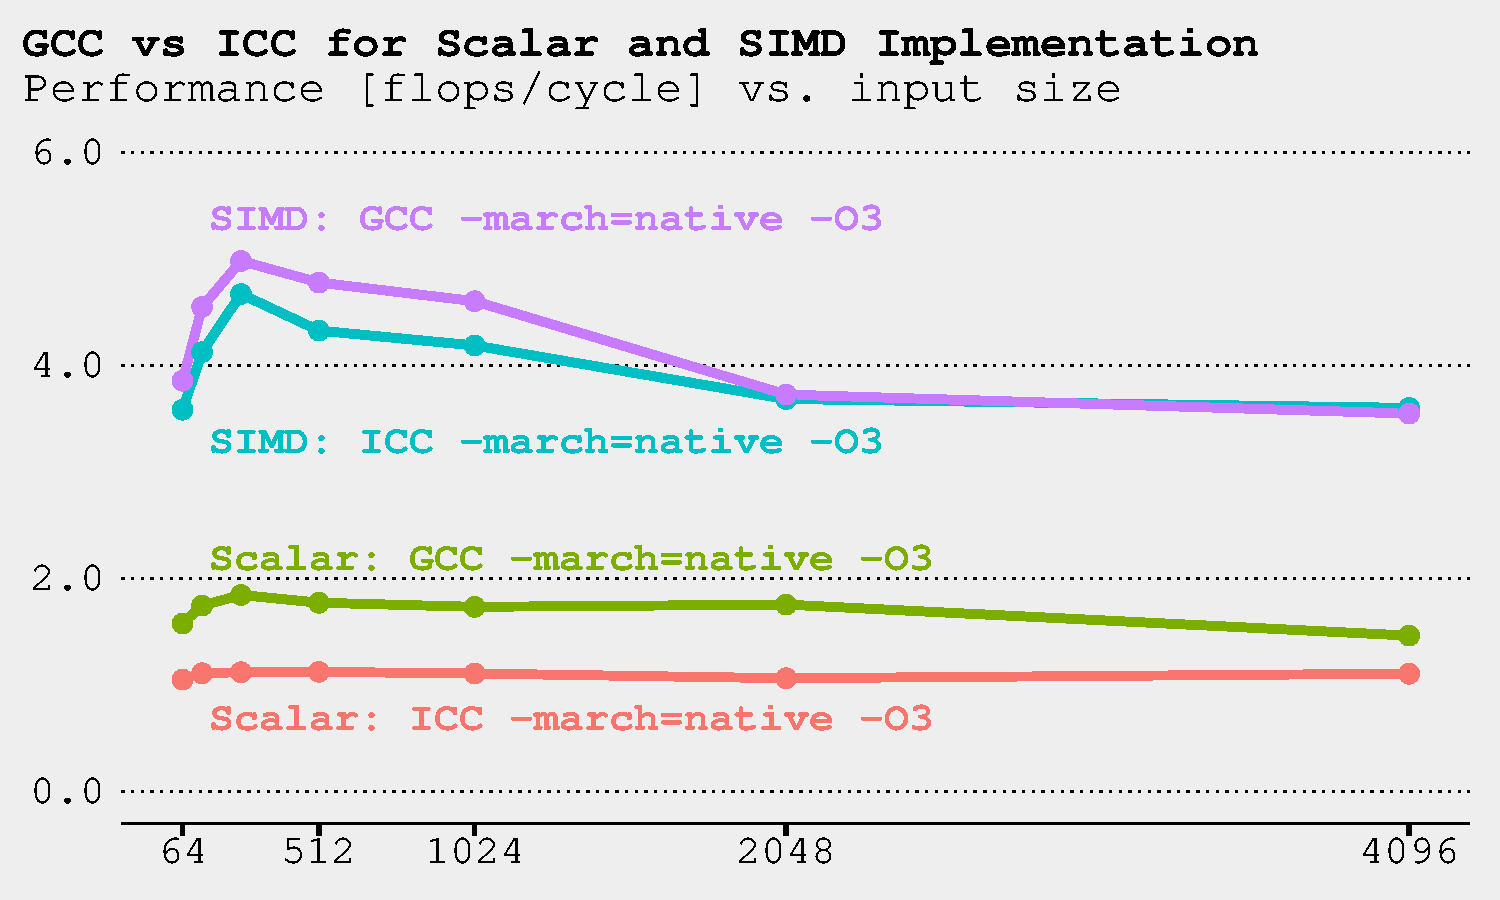
\includegraphics[page=1, width=\linewidth]{performance_gcc_vs_icc}
  \caption{Performance comparison between GCC and ICC with the best scalar and
    SIMD implementation}\label{fig:perf_gcc_vs_icc}
\end{figure}

Because the Intel compiler with various compiler flags did not lead to
improvements, we used gcc with the flags \texttt{-march=native -O3} which
performed best for all the upcoming benchmarks.

\mypar{Performance} The plot in figure~\ref{fig:perf} shows the performance of
our major implementations. As a first result we observe that our baseline
implementation achieves an equal or slightly better performance than the
open-source reference C\texttt{++} implementation~\cite{github-cpp}. Values for
large images are not shown in the plot because the measurements took too much
time.

The optimized scalar implementation which includes precomputations, a better
memory layout and ILP is four times faster than the baseline. The optimizations
become even more apparent when we compare the runtime as in figure
\ref{fig:runtime}. The plot shows that the runtime decreased by several orders
of magnitude and we were finally able to compress larger images in a reasonable
amount of time.

\begin{figure}[H]
  \centering
  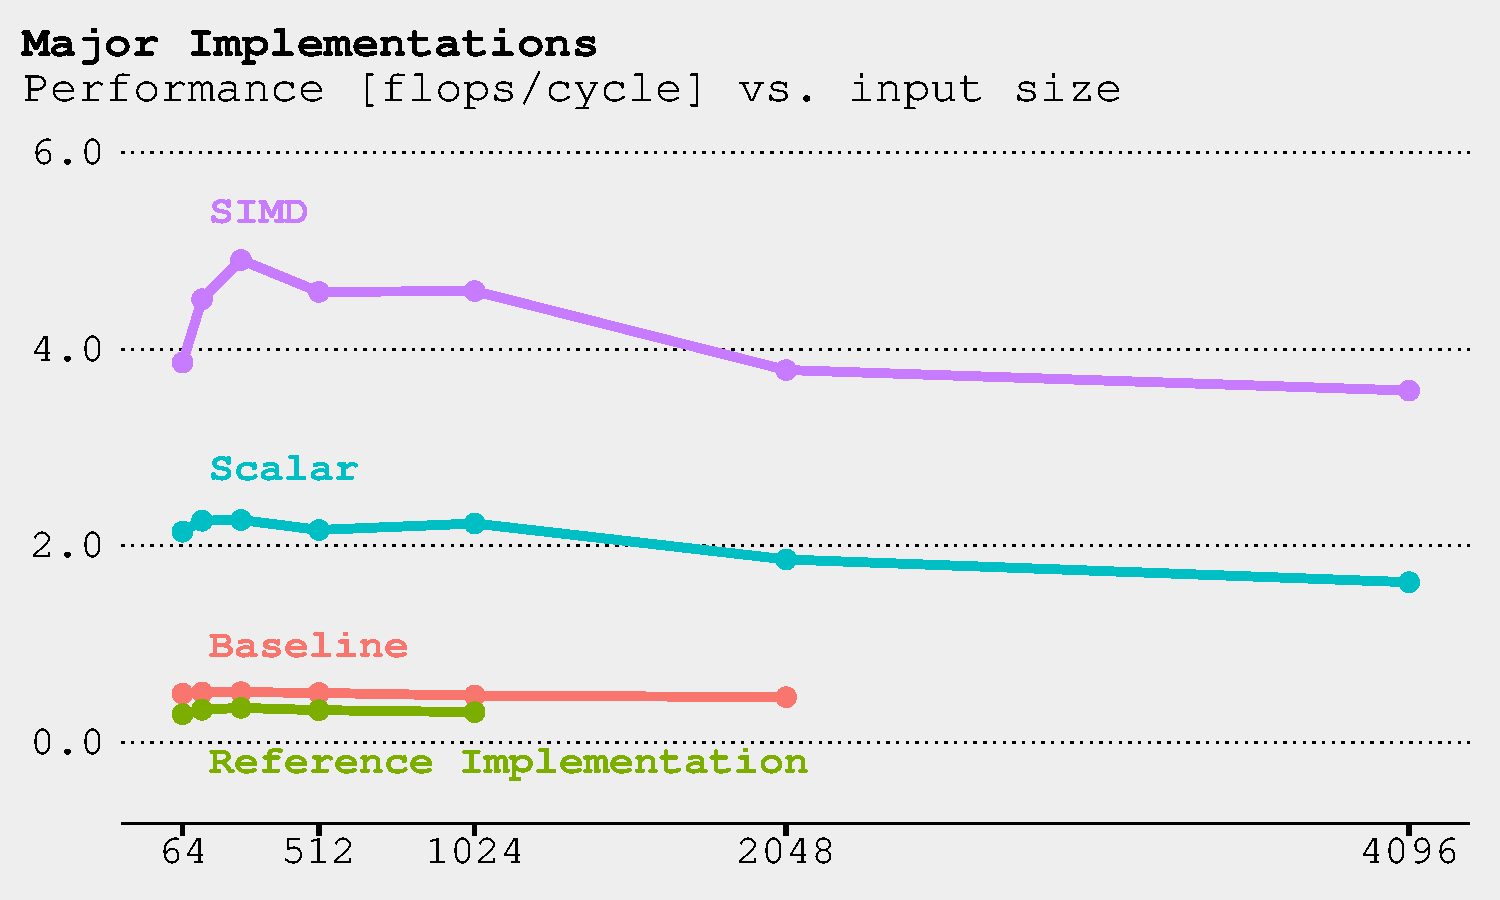
\includegraphics[page=1, width=\linewidth]{performance_major_versions}
  \caption{Performance of our three major implementations and a reference
    implementation from GitHub written in C\texttt{++}}\label{fig:perf}
\end{figure}

\begin{figure}[H]
  \centering
  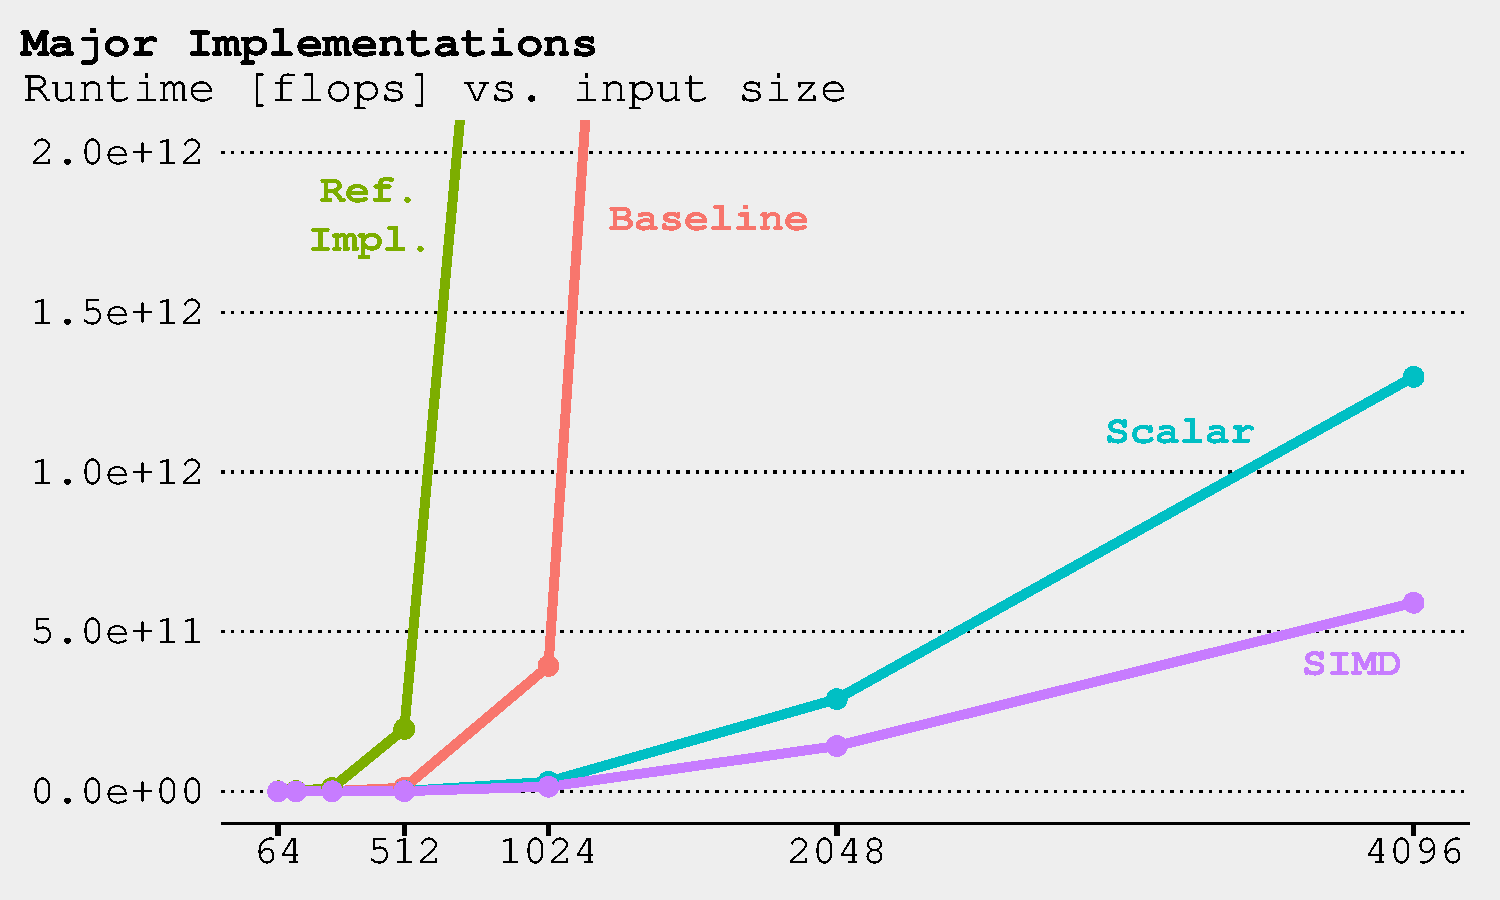
\includegraphics[page=1, width=\linewidth]{runtime_major_versions}
  \caption{Runtime of our three major implementations and a reference
    implementation from GitHub written in C\texttt{++}}\label{fig:runtime}
\end{figure}

\begin{figure}[t]
  \centering
  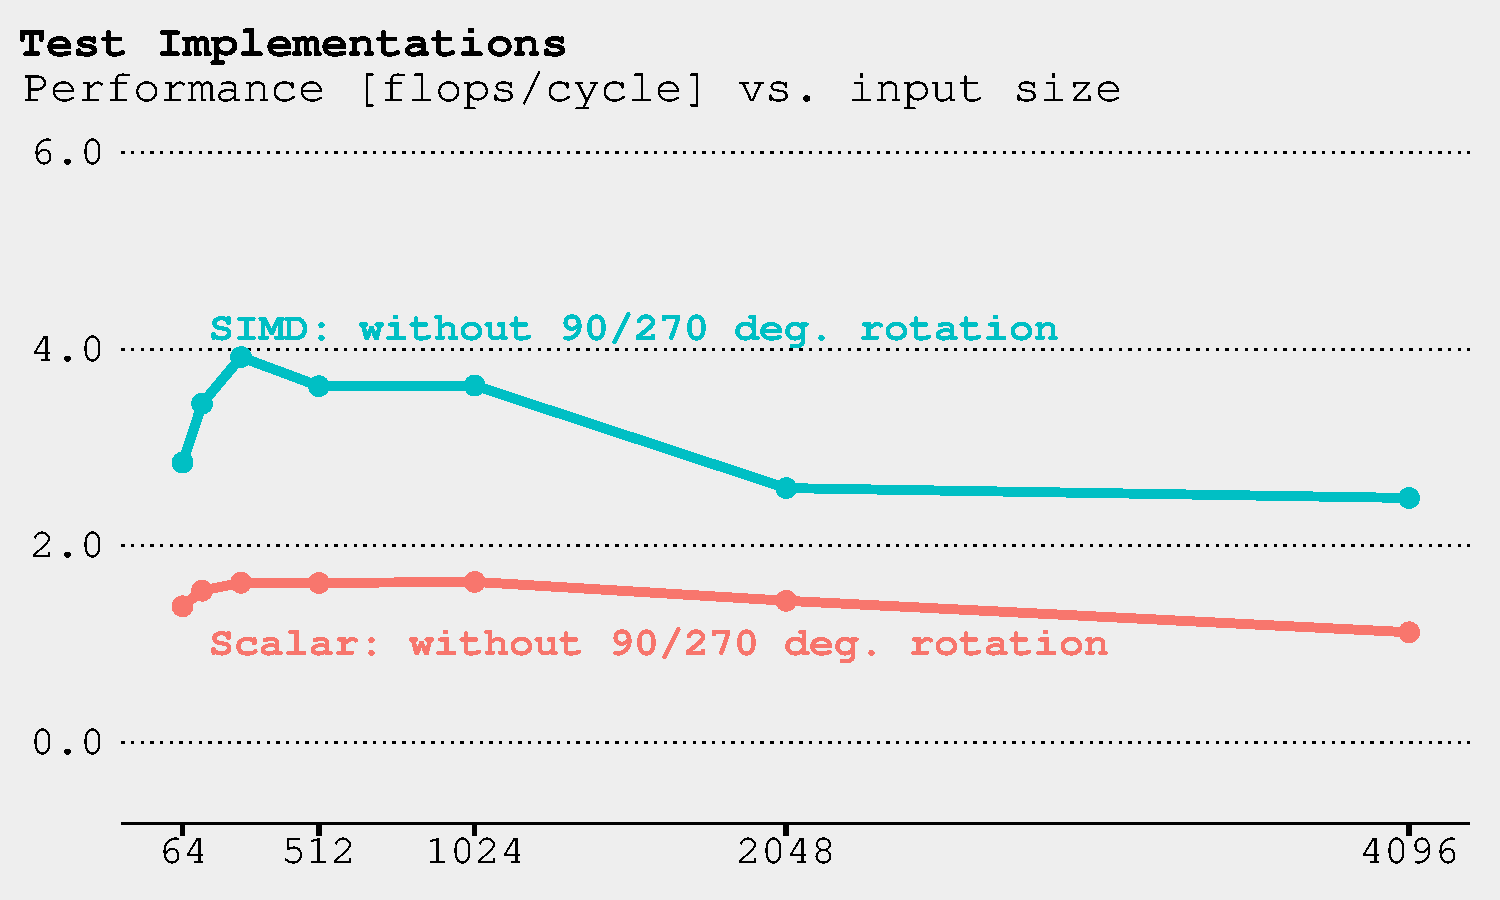
\includegraphics[page=1, width=\linewidth]{performance_norot}
  \caption{Performance Plot without 90/270 degree rotations}\label{fig:perf_40_41}
\end{figure}

As described in section \ref{sec:yourmethod} the initial attempt in vectorizing
the code did not lead to the expected performance improvements. In fact, it
performed just slightly better than the scalar optimized code. We suspected that
the gathering instructions, which are necessary for the rotations, are
responsible for poor performance. To verify this assumption, we removed the
column-wise access to the image i.e. 90/270 degree rotations from the scalar
optimized and the vectorized version. The result of this experiment is shown in
figure \ref{fig:perf_40_41} and one can clearly see how the vectorized code
outperforms the scalar optimized version.

After this experiment, we improved the column-wise access by rotating the range
block instead of the domain block for the 90/270 degree rotations. The improved
vectorized implementation has a performance roughly eight times as high as the
baseline and about twice the performance of the scalar optimized version. The
runtime was also reduced especially for large images.

\section{Conclusions}

With scalar optimizations, our implementation gains a performance speedup
of roughly 4x, whereas the vectorized implementation has a performance speedup
of roughly 8x compared with our straightforward implementation. It is important
to mention that the runtime was decreased significantly and tangibly. Compressing
an image with $2048 \times 2048$ pixels with the baseline implementation takes 
about 2 hours, whereas the vectorized implementation needs 2.5 minutes.

Our fastest implementation with a performance of \\
4 flops/cycle is still 4 times
below the theoretical peak performance of 16 flops/cycle. As the algorithm
in this form is not memory bound, further performance improvements can be expected.

To furthermore boost performance one would also need to apply algorithmic changes. 
Using exhaustive block mapping with a rather large
domain block pool (e.g. with four rotations) is a significant performance
bottleneck which does not necessarily lead to better compression results.

We consider our optimizations to be applicable in all of these more advanced
and mature fractal image compression schemes.

\section{Contributions of Team Members}

\mypar{Jonas} Focused on the baseline implementation and the following scalar optimizations 
(ILP, removal of structs, removal of pointer chasing and decreasing of memory reallocation). 
Helped in prototyping SIMD (especially the four-domain-blocks-a-time approach) 
and contributed to the solution which increased SIMD performance regarding 90 and 270 degree rotations. \\
Wrote a tool to simulate cache access in order to determine tighter memory bounds in the roofline plot. \\
Experimented with block-wise domain/range block traversal.

\mypar{Pascal} \dots

\mypar{Fabian} Added rotations to baseline. Created roofline plot and compared baseline to reference 
implementation. ILP and index optimizations for $\sum_{i=1}^n a_i b_i$ calculation. 

Implemented parts of four-domain-blocks-a-time SIMD (tricky part was error calculcation with 
\verb|blendv| and mask) and participated in bringing the two SIMD approaches together. 
Helped increasing performance regarding 90 and 270 degree rotations.

\mypar{Janis} Changed baseline from C\texttt{++} to C and started with the implementation of a fast queue.
Due to personal problems he withdrew from the project.


% References should be produced using the bibtex program from suitable
% BiBTeX files (here: bibl_conf). The IEEEbib.bst bibliography
% style file from IEEE produces unsorted bibliography list.
% -------------------------------------------------------------------------
\bibliographystyle{IEEEtran}
\bibliography{bibl_conf}

\end{document}
